%%%%%%%%%%%%%%%%%%%%%%%%%%%%%%%%%%%%%%%%%%%%%%%%%%%%%%%%%%%%%%%%%%%%%%
%%                           APPENDIX C
%%%%%%%%%%%%%%%%%%%%%%%%%%%%%%%%%%%%%%%%%%%%%%%%%%%%%%%%%%%%%%%%%%%%%

\chapter{\uppercase {Supplemental Data - Chapter Three}}
\section{Methods extended}
%%%%%%%%%%%%%%%%%%%%%%%%%%%%%%%%%%%%%%%%%%%%%%%%%%%%%%
\begin{longtabu} {X[0.9,c]X[1.1,l]X[1.2,l]X[1,l]X[1,c]}
  \caption{Mouse tissue information by study}\\
  \label{tableC:1}\\
  \toprule
  \textbf{Study} & \textbf{Strain} & \textbf{Tissue} & \textbf{Accession} & \textbf{Read count (million)}\\
  \midrule
  \endhead
  ERP000591 & C57xDBA    & heart        & ERR032227 & 31.0\\
            &            &              & ERR032228 & 8.6 \\
            &            &              & ERR032229 & 30.1\\
            &            &              & ERR032238 & 29.5\\
            &            &              & ERR032230 & 27.8\\
            &            &              & ERR032231 & 31.2\\
            &            & hippocampus  & ERR032232 & 18.8\\
            &            &              & ERR032233 & 33.6\\
            &            &              & ERR032234 & 23.8\\
            &            &              & ERR032235 & 23.2\\
            &            &              & ERR032236 & 22.6\\
            &            &              & ERR032237 & 32.7\\
            &            & liver        & ERR032203 & 28.6\\
            &            &              & ERR032204 & 30.0\\
            &            &              & ERR032205 & 29.3\\
            &            &              & ERR032206 & 30.8\\
            &            &              & ERR032207 & 31.3\\
            &            &              & ERR032208 & 31.4\\
            &            & lung         & ERR032221 & 11.7\\
            &            &              & ERR032222 & 25.8\\
            &            &              & ERR032223 & 23.3\\
            &            &              & ERR032224 & 12.1\\
            &            &              & ERR032225 & 28.4\\
            &            &              & ERR032226 & 18.3\\
  \midrule
  SRP012040 & C57BL/6J   & cerebellum   & SRR567488 & 151 \\
            &            &              & SRR567489 & 145 \\
            &            & cortex       & SRR567480 & 156 \\
            &            &              & SRR032481 & 166 \\
            &            & frontal lobe & SRR567478 & 186 \\
            &            &              & SRR567479 & 159 \\
  \midrule
  SRP017966 & C57xCASTEi & vehicle      & SRR649455 & 94.4\\
            &            &              & SRR649456 & 97.4\\
            &            &              & SRR649457 & 12.9\\
            &            &              & SRR649458 & 10.6\\
            &            &              & SRR649459 & 18.8\\
            &            & topotecan    & SRR649460 & 102 \\
            &            &              & SRR649461 & 113 \\
            &            &              & SRR649462 & 16.9\\
            &            &              & SRR649463 & 8.8 \\
            &            &              & SRR649464 & 14.6\\
  \midrule
  SRP033200 & Aldh1l1-EGFP & astrocytes  & SRR1033783 & 29.6\\
            &              &             & SRR1033784 & 32.0\\
            & NA           & neurons     & SRR1033785 & 37.9\\
            &              &             & SRR1033786 & 33.9\\
            &              & oligodendrocyte precursor cells & SRR1033787 & 32.2\\
            &              &             & SRR1033788 & 32.5\\
            &              & newly formed oligodendrocytes & SRR1033789 & 32.1\\
            &              &             & SRR1033790 & 30.5\\
            &              & myelinating oligodendrocytes & SRR1033791 & 33.4\\
            &              &             & SRR1033792 & 29.7\\
            &              & microglia   & SRR1033793 & 29.2\\
            &              &             & SRR1033794 & 30.0\\
            & Tie2-EGFP    & endothelial cells & SRR1033795 & 36.5\\
            &              &             & SRR1033796 & 33.8\\
  \bottomrule
\end{longtabu}
%%%%%%%%%%%%%%%%%%%%%%%%%%%%%%%%%%%%%%%%%%%%%%%%%%%%%%
\pagebreak

%%%%%%%%%%%%%%%%%%%%%%%%%%%%%%%%%%%%%%%%%%%%%%%%%%%%%%
\begin{longtabu} to \textwidth {X[1.5,l]X[2.5,l]X[1,c]}
  \caption{\emph{Ube3a} Mechanism Primer List}\\
  \label{primerList}\\
  \toprule
  \textbf{Primer Name} & \textbf{Sequence}       & \textbf{Reference}\\
  \midrule
  \endhead
  ActB Fwd            & GGCTGTATTCCCCTCCATCG     & \cite{Meng2012}\\
  ActB Rev            & CCAGTTGGTAACAATGCCATGT   & \cite{Meng2012}\\
  Map2 Fwd            & GCCAGCCTCAGAACAAACAG     & \\
  Map2 Rev            & AAGGTCTTGGGAGGGAAGAAC    & \\
  Ube3a-AS 1 Fwd      & GGCTCTACGAGAAGCTGACTG    & \\
  Ube3a-AS 1 Rev      & GTTGCCATCACCTTCAGTTC     & \\
  Ube3a-AS 3 Fwd      & GCTACATGCTAGGCCCTAATG    & \\
  Ube3a-AS 3 Fwd      & ATGGAGTTCTCTTGACCAAGTC   & \\
  Ube3a$^{YFP}$ Fwd   & GGTGACTAATGAATCGCCCTTA   & \\
  Ube3a$^{YFP}$ Rev   & GTTTACGTCGCCGTCCAG        & \\
  \midrule
  Iso4 3'RACE Fwd     & CAAGGCTGACTTCAAACTCAGATA & \\
  Iso4 3'RACE nxt\footnotemark Fwd & TCTCCTGTTTCTGCTTTCTGAG   & \\
  Ube3a Exon 4 Fwd    & ACCAGGAGAATCCCAGTCTGA    & \\
  Ube3a Exon 4.1 Rev  & ATTTGATGCTGGTCATGGTG     & \\
  Ube3a Exon 5 Rev    & TCATTCGTGCAGGCCTCATT     & \\
  \bottomrule
\end{longtabu}
%%%%%%%%%%%%%%%%%%%%%%%%%%%%%%%%%%%%%%%%%%%%%%%%%%%%%%
\footnotetext{nxt: nested}

\section{Gene prediction}
\subsection{Splicing into \textit{Ube3a} exon 4.1}

%%%%%%%%%%%%%%%%%%%%%%%%%%%%%%%%%%%%%%%%%%%%%%%%%%%%%%
\begin{sidewaysfigure}
  \centering
  \resizebox{\linewidth}{!}{
    \begin{tikzpicture}[every label/.style={font=\Large\bfseries}, pic/.style={inner sep=0pt}]
      \node[pic] (top)              {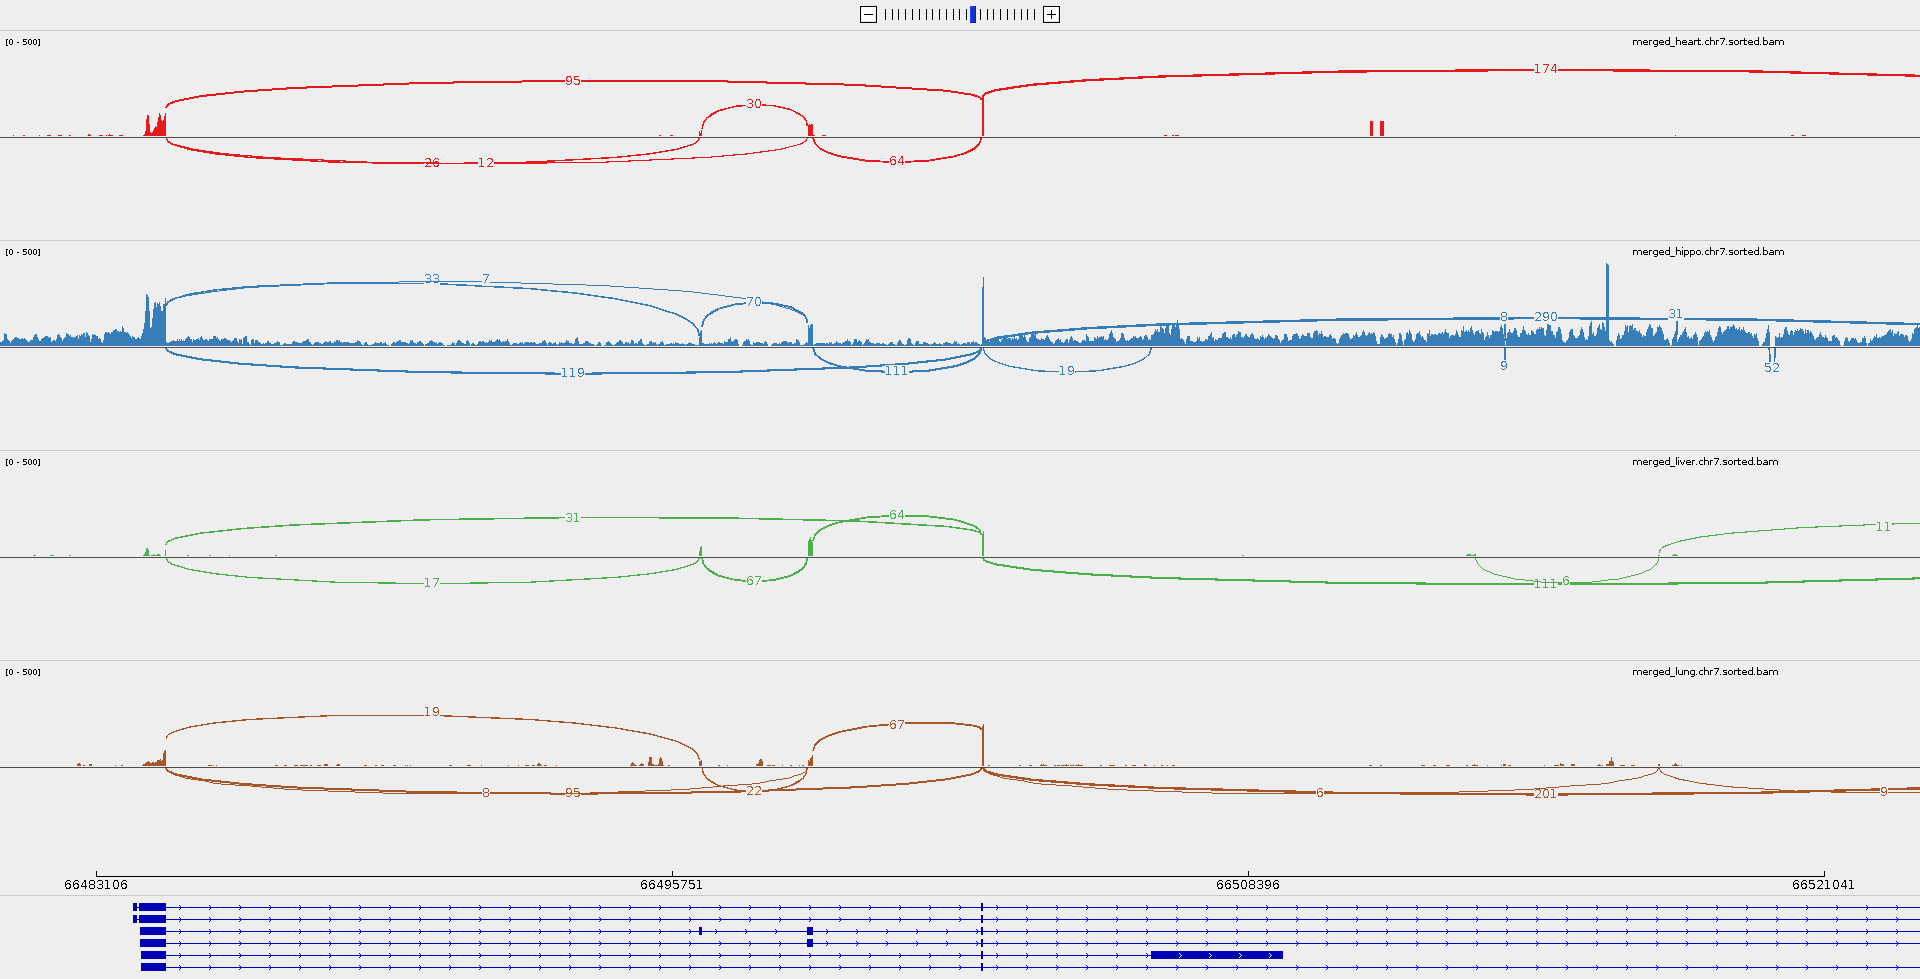
\includegraphics{figures/mouse.sense.sashimi.compare.png}};
    \end{tikzpicture}
  }
  \caption{Sashimi plot comparing heart (red), hippocampus (blue), liver (red), and lung (brown) forward strand demonstrating splicing into novel exon 4.1 only in the brain. Exon coverage of 0 to 500, minimal junction coverage = 5, max junction coverage = 1000.}
  \label{sense tissue splicing}
\end{sidewaysfigure}
%%%%%%%%%%%%%%%%%%%%%%%%%%%%%%%%%%%%%%%%%%%%%%%%%%%%%%

%%%%%%%%%%%%%%%%%%%%%%%%%%%%%%%%%%%%%%%%%%%%%%%%%%%%%%
\begin{sidewaysfigure}
  \centering
  \resizebox{\linewidth}{!}{
    \begin{tikzpicture}[every label/.style={font=\Large\bfseries}, pic/.style={inner sep=0pt}]
      \node[pic] (top)              {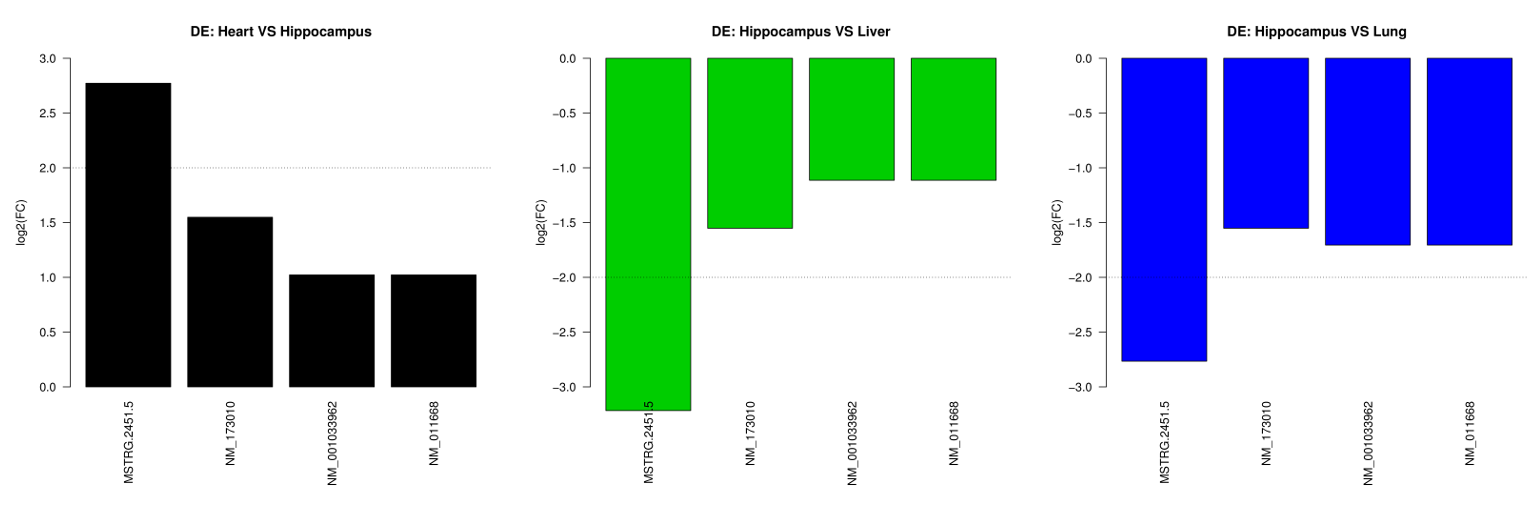
\includegraphics{figures/mouse.sense.log2FC.comparison.png}};
    \end{tikzpicture}
  }
  \caption{Log2 fold-change plots of the four potential isoforms comparing heart, liver, and lung  to hippocamus.}
  \label{sense tissue fold-change}
\end{sidewaysfigure}
%%%%%%%%%%%%%%%%%%%%%%%%%%%%%%%%%%%%%%%%%%%%%%%%%%%%%%

%%%%%%%%%%%%%%%%%%%%%%%%%%%%%%%%%%%%%%%%%%%%%%%%%%%%%%
\begin{sidewaysfigure}
  \centering
  \resizebox{\linewidth}{!}{
    \begin{tikzpicture}[every label/.style={font=\Large\bfseries}, pic/.style={inner sep=0pt}]
      \node[pic] (top)              {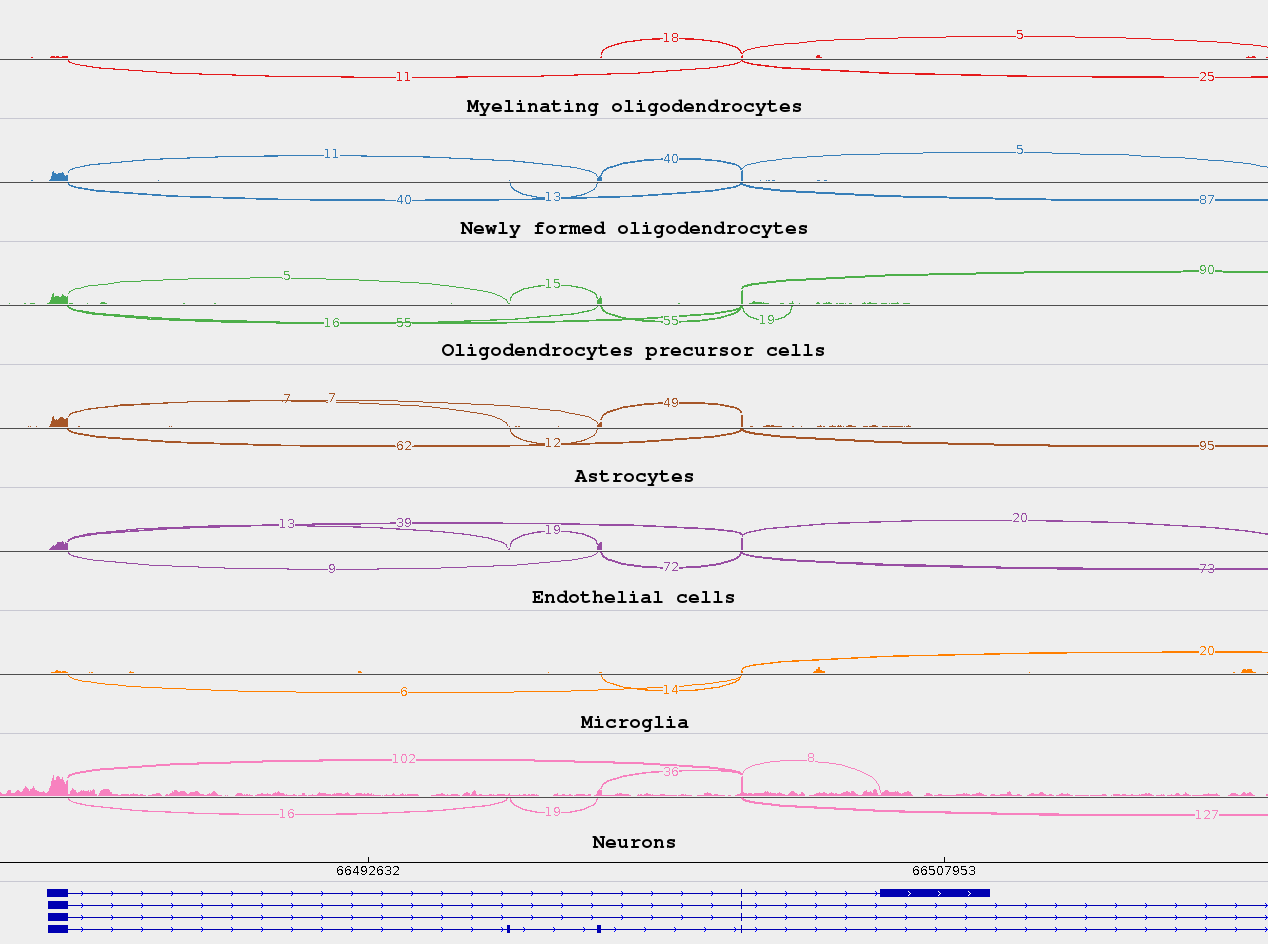
\includegraphics{figures/mouse.sense.sashimi.celltype.png}};
    \end{tikzpicture}
  }
  \caption{Sashimi plot comparing different cell populations in the mouse cerebral cortex. Forward strand only, with exon coverage = 0 to 500, minimal junction coverage = 5, max junction coverage = 1000.}
  \label{sense celltype splicing}
\end{sidewaysfigure}
%%%%%%%%%%%%%%%%%%%%%%%%%%%%%%%%%%%%%%%%%%%%%%%%%%%%%%

%%%%%%%%%%%%%%%%%%%%%%%%%%%%%%%%%%%%%%%%%%%%%%%%%%%%%%
\begin{sidewaysfigure}
  \centering
  \resizebox{\linewidth}{!}{
    \begin{tikzpicture}[every label/.style={font=\Large\bfseries}, pic/.style={inner sep=0pt}]
      \node[pic] (top)              {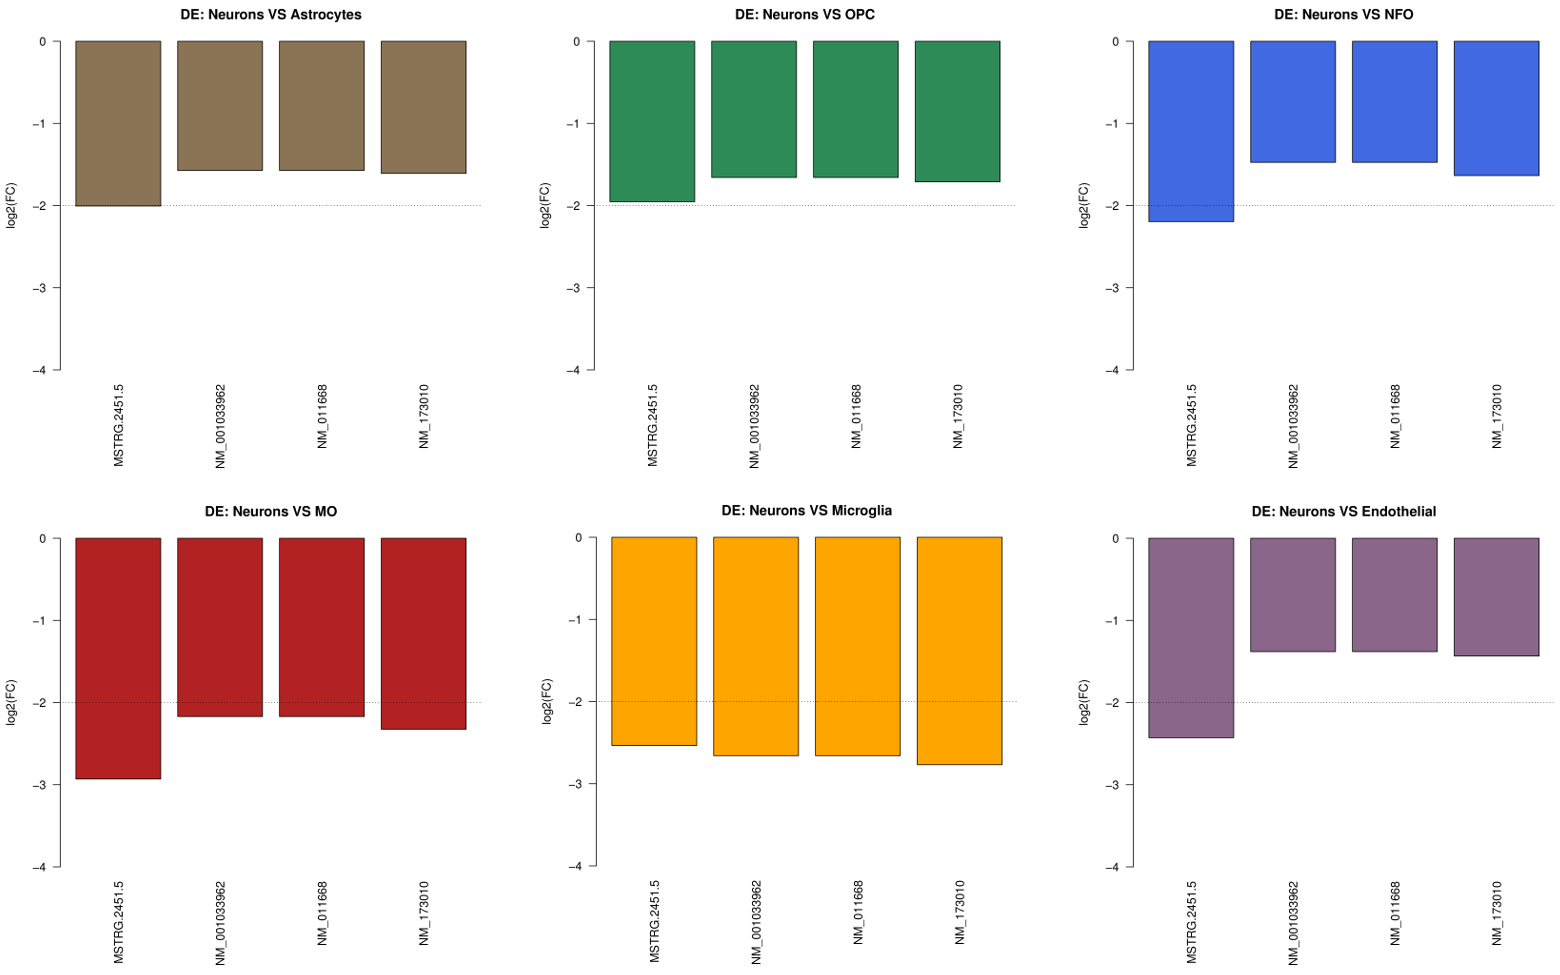
\includegraphics{figures/mouse.sense.log2FC.celltype.png}};
    \end{tikzpicture}
  }
  \caption{Log2 fold-change plots of the four potential isoforms comparing other cell population in the mouse cerebral cortex to neurons.}
  \label{sense celltype fold-change}
\end{sidewaysfigure}
%%%%%%%%%%%%%%%%%%%%%%%%%%%%%%%%%%%%%%%%%%%%%%%%%%%%%%

\pagebreak
\section{Gene structure analysis}
\begingroup\small\begin{verbatim}
______________________________________________________________________
Sequence    5:   MSTRG.2451.5, from 1 to 3512.
**********************************************************************
Query protein sequence    2 (File: NP_766598.1)
  1 MKRAAAKHLI ERYYHQLTEG CGNEACTNEF CASCPTFLRM DNNAAAIKAL ELYKINAKLC
 61 DPHPSKKGAS SAYLENSKGA SNNSEIKMNK KEGKDFKDVI YLTEEKVYEI YEFCRESEDY
121 SPLIRVIGRI FSSAEALVLS FRKVKQHTKE ELKSLQEKDE DKDEDEKEKA ACSAAAMEED
181 SEASSSRMGD SSQGDNNVQK LGPDDVTVDI DAIRRVYSSL LANEKLETAF LNALVYLSPN
241 VECDLTYHNV YTRDPNYLNL FIIVMENSNL HSPEYLEMAL PLFCKAMCKL PLEAQGKLIR
301 LWSKYSADQI RRMMETFQQL ITYKVISNEF NSRNLVNDDD AIVAASKCLK MVYYANVVGG
361 DVDTNHNEED DEEPIPESSE LTLQELLGDE RRNKKGPRVD PLETELGVKT LDCRKPLISF
421 EEFINEPLND VLEMDKDYTF FKVETENKFS FMTCPFILNA VTKNLGLYYD NRIRMYSERR
481 ITVLYSLVQG QQLNPYLRLK VRRDHIIDDA LVRLEMIAME NPADLKKQLY VEFEGEQGVD
541 EGGVSKEFFQ LVVEEIFNPD IGMFTYDEAT KLFWFNPSSF ETEGQFTLIG IVLGLAIYNN
601 CILDVHFPMV VYRKLMGKKG TFRDLGDSHP VLYQSLKDLL EYEGSVEDDM MITFQISQTD
661 LFGNPMMYDL KENGDKIPIT NENRKEFVNL YSDYILNKSV EKQFKAFRRG FHMVTNESPL
721 KYLFRPEEIE LLICGSRNLD FQALEETTEY DGGYTRESVV IR-

Predicted gene structure (within gDNA segment 1 to 3512):
Exon 1, 3: 64 (62 n); Protein 745, 762 (18 aa); score: 0.027

MATCH	MSTRG.2451.5+	NP_766598.1	0.027	62	0.027	P
PGS_MSTRG.2451.5+_NP_766598.1	(3  64)

Alignment:
GAGCCCTCGC CCGGCAGGGT TGGCGCGCGC TGCCTGTCGG GATACTCGGT CCGCC-CACC 61
 E  P  S   P  G  R  V   G  A  R   C  L  S   G  Y  S  V   R     T  
 |     +                |  .            .   .        +   |        
 E  E  T   T  E  Y  D   G  G  Y   T  R  E   S  V  V  I   R  -  -  762
TAG       64
 * 
 *       763
__________________________________________________________________
\end{verbatim}
\endgroup

\section{3'RACE sequences}
\begingroup\tiny
\begin{verbatim}
>A01_4b-4.seq 
TGCACGCAAGCTCGATAACCCTCACTAAAGGGACTAGTCCTGCAGGTTTAAACGAATTCGCCCTTTCTCCTGTTTCTGCTTTCTGAGTGTGAGATTAAAGGTGTTGTACCACCATGACCA
GCATCAAATTCATGAGAAAAAAAATTCTTTACCTTTCTAATCATCTAAGAAATGAAACAACAGTGAGATACTACTTCCTACCTGCTAGAATATATGAATGTTCATGTTGGTGAGGTTGTA
AGCAAACAGAAATCTTGTACACAGTTGTTTGGAATGTAAATTAGATCGATTATGGAAAATAACAGGTTCCTAAAAATTGCAATGACCTAGCAATTGTATTATAGAAATATATAGTGTGTT
ATAAGAGATACCTGCAGTTTAATTTTGATTGCAGCATTAATTAAACAAAATGCAGAAATAAACCAGTGTTTGTCAGTG

>B01_4b-5.seq
TGACGCCGCTCGCATAACCCTCACTAAAGGGACTAGTCCTGCAGGTTTAAACGAATTCGCCCTTTCTCCTGTTTCTGCTTTCTGAGTGTGAGATTAAAGGTGTTGTACCACCATGACCA
GCATCAAATTCATGAGAAAAAAAATTCTTTACCTTTCTAATCATCTAAGAAATGAAACAACAGTGAGATACTACTTCCTACCTGCTAGAATATATGAATGTTCATGTTGGTGAGGTTGT
AAGCAAACAGAAATCTTGTACACAGTTGTTTGGAATGTAAATTAGATCGATTATGGAAAATAACAGGTTCCTAAAAATTGCAATGACCTAGCAATTGTATTATAGAAATATATAGTGTG
TTATAAGAGATACCTGCAGTTTAATTTTGATTGCAGCATTAATTAAACAAAATGCAGAAATAAACCAGTGTTTGTCAGTGGCTAAACAAATAAAAATTGACATATATGATGATGTAATT
TTTCGCCATTAAAATTTTTTTCTGAAATCTTATGTCGGTGACAACATGGATGGAAATGATCCTTTATATTTTCAAAGAAATAAATCAGCACAAAAACAGGTAGTGCATCATCTTCCTGT
ACATAGACTGTAAAAACATTCTAAAAATTGTTTGTTACTTAGAGTAGAATAAATGATAGACATAAAAAATGCAAAATGAATAGAATGTAGTTCAGGACCAAAATTGTAGAGCATGGTGA
CTTCTTTCTGTATATTTTCTTGAATATCACTAAAAGTCAACTATTAAGTATATGTGCAAAAAGTGCTATGTTAGAATTTATAAACTCATTTGATGTATCACTTTTGCATATGATAATAT
ATGTAGTTCTTATTTGTCAATGAAAATAAAAACTTTGGGAAAAACAAAAAAAAAAAAAAAAAAAGATTAAGAATAAAAAAAAAAAAAAAAAAGTCTAGTCGACGCGTGGCACAAAGGGC
GAATTTCGCGGCCGCTAAATTTCAATTCGCCCTATAGTGAGTCGTATAACAATTCACTGGCCGTCGTTTTACAACGTCGTGACTGAAAAACCTGCCGTTACCAACTTAATCGCCTTGAC
AGCACATCCCCCATTACGCAAC

>C01_4b-6.seq
TCCACGCCCGCCTTAGATAACCCCTCACTAAAGGGACTAGTTCCTGCAGGTTTAAACCGAATTCGCCCTTTCTCCTGTTTCTGCTTTCTGAGTGTGAGATTAAAGGTGTTGTACCACCA
TGACCAGCATCAAATTCATGAGAAAAAAAATTCTTTACCTTTCTAATCATCTAAGAAATGAAACAACAGTGAGATACTACTTCCTACCTGCTAGAATATATGAATGTTCATGTTGGTGA
GGTTGTAAGCAAACAGAAATCTTGTACACAGTTGTTTGGAATGTAAATTAGATCGATTATGGAAAATAACAGGTTCCTAAAAATTGCAATGACCTATCAATTGTATTATCTAGAAATAT
ATACTGTGT

>F02_4b-1.seq
TGAGCCGCTCGTATTAACCCTCACTAAAGGGACTAGTCCTGCAGGTTTAAACGAATTCGCCCTTGGCCACGCGTCGACTAGTACTTTTTTTTTTTTTTTTTTTTTCCAAAGTTTTTATT
TTCATTGACAAATAAGAACTACATATATTATCATATGCAAAAGTGATACATCAAATGAGTTTATAAATTCTAACATAGCACTTTTGCACATATACTTAATAGTTGACTTTTAGTGATAT
TCAAGAAAATATACAGAAAGAAGTCACCATGCTCTACAATTTTGGTCCTGAACTACATTCTATTCATTTTGCATTTTTTATGTCTATCATTTATTCTACTCTAAGTAACAAACAATTTT
TAGAATGTTTTTACAGTCTATGTACAGGAAGATGATGCACTACCTGTTTTTGTGCTGATTTATTTCATTGAAAATATAAAGGATCATTTCCATCCATGTTGTCACCGACATAAGATTTC
AGAAAAAAATTTTAATGGCGAAAAATTACATCATCATATATGTCAATTTTTATTTGTTTAGCCACTGACAAACACTGGTTTATTTCTGCATTTTGTTTAATTAATGCTGCAATCAAAAT
TAAACTGCAGGTATCTCTTATAACACACTATATATTTCTATAATACAATTGCTAGGTCATTGCAATTTTTAGGAACCTGTTATTTTCCATAATCGATCTAATTTACATTCCAAACAACT
GTGTACAAGACTTCTGTTTGCTTACAACCTCACCAACATGAACATTCATATATTCTAGCAGGTAGGAAGTAGTATCTCACTGTTGTTTCATTTCTTAGATGATTAGAAAGGTAAAGAAT
TTTTTTTCTCATGAATTTGATGCTGGTCATGGTGGTACAACACCTTTAATCTCACACTCAGAAAGCAGAAACAGGAGAAAGGGCGAATTCGCGGCCCGCTAAATTCAATTCGCCCTATA
GTGAGTCGTATTACAATTTCACTGGCCCGTCGTTTTACACGTCGTGACTGGAAACCCTGCGTACCACTATTCGCTGCAGCACATCCCCATTCGCAGCTGCGTATAGCGAGAGCCCGCAC
GATCGCCTCACAGGTTGCCAGCCTATACGTACGGCAGTAGTTACCTTAGAGAAGCCGTTATCGACTGTTTATGA

>G02_4b-2.seq
TGAGCCGCTCTATTAACCCTCACTAAAGGGACTAGTCCTGCAGGTTTAAACGAATTCGCCCTTTCTCCTGTTTCTGCTTTCTGAGTGTGAGATTAAAGGTGTTGTACCACCATGACCAG
CATCAAATTCATGAGAAAAAAAATTCTTTACCTTTCTAATCATCTAAGAAATGAAACAACAGTGAGATACTACTTCCTACCTGCTAGAATATATGAATGTTCATGTTGGTGAGGTTGTA
AGCAAACAGAAATCTTGTACACAGTTGTTTGGAATGTAAATTAGATCGATTATGGAAAATAACAGGTTCCTAAAAATTGCAATGACCTAGCAATTGTATTATAGAAATATATAGTGTGT
TATAAGAGATACCTGCAGTTTAATTTTGATTGCAGCATTAATTAAACAAAATGCAGAAATAAACCAGTGTTTGTCAGTGGCTAAAAAAAAAAAAAAAAAAAAAAAAAAAAAAAAAAAAT
AAAAAAAAAAAAAAAAAAAAGGTACTAGTCGACCCGTGGCCAAGGGCAAATTCGCGGCCGCTAAATTCAATTCCCCCTATAGTGAGTCGTATTACAATTCACTGGCCGTCGTTTTACAA
CGTCGGGACTGGGAAAACCCTGGCGTTCCCAAACTTAATCGCCTTGCAGCACATCCCCCTTTCGCCAGCTGGCGTAATAGCGAAAAGGCCCGCACCGTTCGCCCCTTCCCAACATTTGC
GCAGCCTTTTCGTACGGGAGTTTAAGGGTTTACACCCTATAAAAAAAGAGAGCCGTTTTCTTTTTGTTTGGGGATGTACAGAATTGATTTTTTTTGACCCCCCGGGGCGACGGGATGGG
GGAATCCCCCTGGCCAGTGCCCGTTTGCTGTCAAATAAAGTTCTCCCGTGAACTTTACCCCGGGGGGCATATCCGGGATTGAAAGCTGGCCCATTATGTCCCCCCATTTGGCCATGGTG
CCGGTCTCCCTTTATCGGGGAAGAAAATGGCTGATCTCAGCCCACCGCGAAATGACATTCAAACGCCTTAACCTGATGTTTCTGGGGAAATATTA

>H02_4b-3.seq
TGCAGCCGCTCGTATTAACCCCTCACTAAAGGGACTAGTCCTGCAGGTTTAAACGAATTCGCCCTTTCTCCTGTTTCTGCTTTCTGAGTGTGAGATTAAAGGTGTTGTACCACCATGAC
CAGCATCAAATTCATGAGAAAAAAAATTCTTTACCTTTCTAATCATCTAAGAAATGAAACAACAGTGAGATACTACTTCCTACCTGCTAGAATATATGAATGTTCATGCTGGTGAGGTT
GTAAGCAAACAGAAATCTTGTACACAGTTGTTTGGAATGTAAATTAGATCGATTATGGAAAATAACAGGTTCCTAAAAATTGCAATGACCTAGCAATTGTATTATAGAAATATATAGTG
TGCTATAAGAGATACCTGCAGTTTAATTTTGATTGCAGCATTAATTAAACAAAATGCAGAAATAAACCAGTGTTTGTCAGTGGCTAAACAAATAAAAATTGACATATATGATGATGTAA
TTTTTCGCCATTAAAATTTTTTTCTGAAATCTTATGTCGGTGACAACATGGATGGAAATGATCCTTTATATTTTCAATGAAATAAAATCAGCACAAAAAACAGGTAGTGCATCATCTTC
CTGTACATAGACTGTAAAAAACATTCTAAAAAATTGTTTGTTACTTAGAGTAGAATAAATGATAGACATAAAAATGCAAATGAAAT
\end{verbatim}
\endgroup

\section{SNP analysis}
%%%%%%%%%%%%%%%%%%%%%%%%%%%%%%%%%%%%%%%%%%%%%%%%%%%%%%
\begin{figure} [ht]
  \centering
  \resizebox{\linewidth}{!}{
    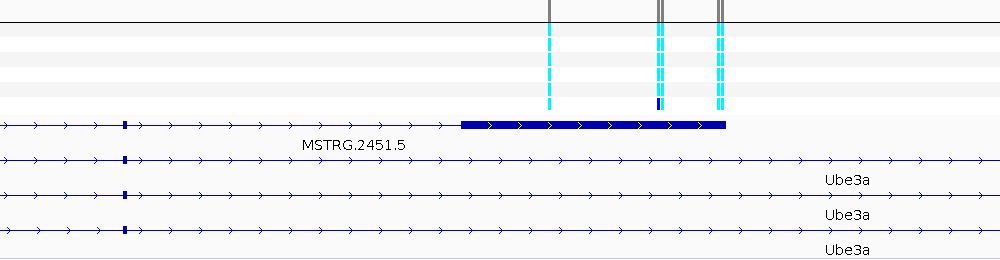
\includegraphics{figures/informative_snps.png}
  }
  \caption{Five informative snps located within exon 4.1. Paternal allele specific expression.}
  \label{informative snps}
\end{figure}
%%%%%%%%%%%%%%%%%%%%%%%%%%%%%%%%%%%%%%%%%%%%%%%%%%%%%%
\pagebreak
\section{Temporal regulation of isoform 4}
%%%%%%%%%%%%%%%%%%%%%%%%%%%%%%%%%%%%%%%%%%%%%%%%%%%%%%
\begin{longtabu} {X[1,c]X[0.9,c]X[0.9,c]X[1,c]X[1.6,c]}
  \caption{Mouse tissue information by study}\\
  \label{tableC:1}\\
  \toprule
  \textbf{Study} & \textbf{Strain} & \textbf{Tissue} & \textbf{Accession} & \textbf{Read count (million)}\\
  \midrule
  \endhead
  SRP048593 & C57BL/6J     & E18-hippo   & SRR1772425 & 41.3\\
            &              &             & SRR1772429 & 34.9\\
            &              & P1-hippo    & SRR1772426 & 38.5\\
            &              &             & SRR1772430 & 34.6\\
            &              & P10-hippo   & SRR1772427 & 34.1\\
            &              &             & SRR1772431 & 41.1\\
            &              & P30-hippo   & SRR1772428 & 43.4\\
            &              &             & SRR1772432 & 41.8\\
  \bottomrule
\end{longtabu}
%%%%%%%%%%%%%%%%%%%%%%%%%%%%%%%%%%%%%%%%%%%%%%%%%%%%%%

Temporal hippocampal RNA-seq datasets were extracted from E18, P1, P10 and P30 mice \cite{You2015}. RNA-seq data analyzed with Illumina HiSeq 2500 platform as single-end, stranded reads.

%%%%%%%%%%%%%%%%%%%%%%%%%%%%%%%%%%%%%%%%%%%%%%%%%%%%%%
\begin{sidewaysfigure}
  \centering
  \resizebox{\linewidth}{!}{
    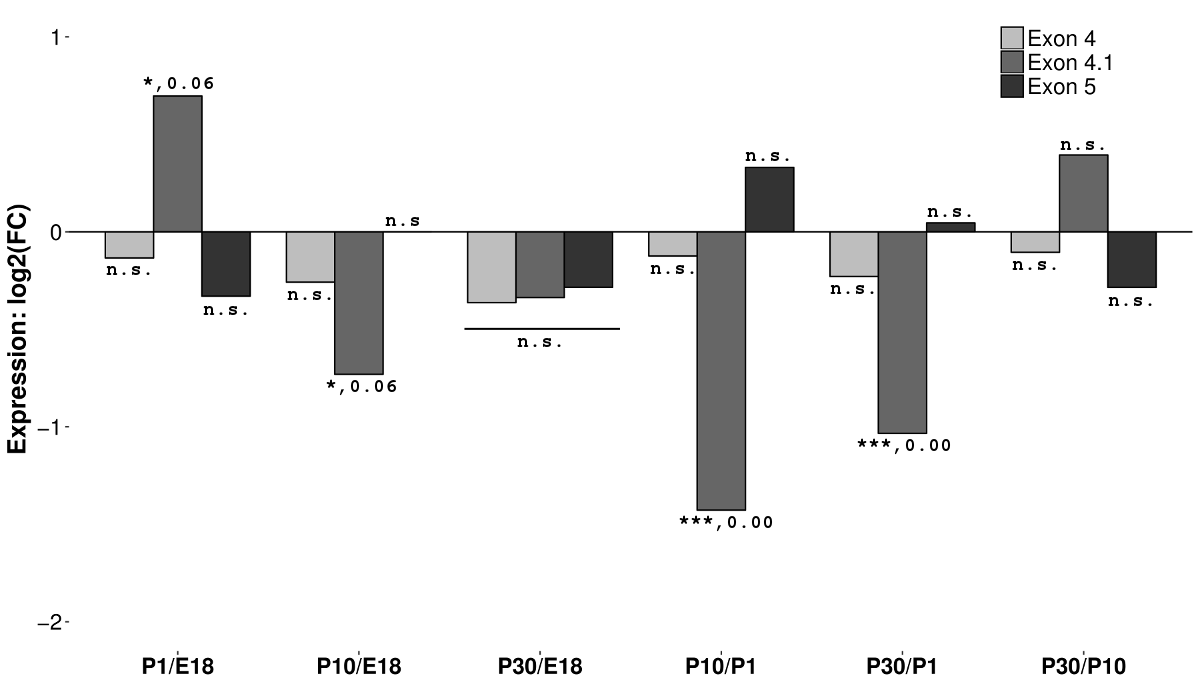
\includegraphics{figures/supplemental.temporal.sense.png}
  }
  \caption{Neuron-specific \textit{Ube3a} isoform 4 is temporally regulated.}
  \label{temporal sense expression}
\end{sidewaysfigure}
%%%%%%%%%%%%%%%%%%%%%%%%%%%%%%%%%%%%%%%%%%%%%%%%%%%%%%
